% uncomment to compile individually
% \DocumentMetadata{
%     lang=en-US,
%     tagging=on,
%     pdfversion=2.0,
%     pdfstandard=ua-2,
%     tagging-setup={math/setup=mathml-SE},
%     colorprofiles={
%         A = sRGB.icc, %or longer GTS_PDFA1 = sRGB.icc
%         X = sRGB.icc,
%         ISO_PDFE1 = sRGB.icc
%     },
%     % pdftitle={Lecture notes - accessibility test},
%     % pdfauthor={Silas Mitchell}
% }

\documentclass{article}
\usepackage[]{notes}

\begin{document}

\setcounter{section}{2}
\setcounter{subsection}{1}

\subsection{Solving linear equations}

\subsubsection{Solving equations of 1 variable}

\begin{definition}{(Mathematical equation)}{def:equation}
    An equation is a statement that two quantities are equal. We call an equation a linear equation of one variable if it can be rearranged to the form $ax+b=0$, where $a$ and $b$ are numbers with $a\neq 0$ and $x$ is the variable.

    Solving a linear equation of 1 variable means finding the value of $x$ that makes the two sides equal.
\end{definition}

\begin{process}{Solving a linear equation}{process:solve_equation}
    In order to solve a linear equation, we are allowed to perform certain operations:
    \begin{itemize}
        \item Add/subtract something from both sides\\
        Ex: if we know $x-5=17$, we can add 5 to both sides to get $x=17+5$
        \item Multiply/divide both sides by the same thing\\
        Ex: if we know $\frac{3}{4}x=6$, we can divide both sides by $\frac{3}{4}$ (same as multiplying by $\frac{4}{3}$) to get $x=6\cdot\frac{4}{3}=8$.
        \item Replace a quantity with something equal\\
        Ex: if we know $a=9$, then we could rewrite $a$ to get $x+a=19x-a$ as $x+9=19x-9$
    \end{itemize}
    Once we have solved for the variable, we can substitute that value into the original equation and simplify both sides to check our answer.
\end{process}

% \includegraphics[width=6.5in]{Textbook_Mandatory_Examples/Exam1/2.2/2.2.2.png}
\begin{example}{(Textbook 2.2 ex 2)}{ex:2.2.3}
    Solve $3(2x-5)=10-(x+5)$. Check your answer.
\end{example}
\begin{solution}
    First we need to solve for $x$. We will simplify both sides to the form $ax+b$, then get all $x$ terms together and all constants together, then divide both sides by the coefficient on $x$.
    \begin{align*}
        3(2x-5)&=10-(x+5)\\
        3\cdot 2x + 3 \cdot (-5) &= 10 -x -5 && \text{Distribute on both sides} \\
        6x-15 &= -x + 5 && \text{Evaluate $\times$ on left, and combine constants on right with $+$} \\
        +x \phantom{-15} &\quad +x && \text{Cancel $-x$ on right by adding $x$ to both sides}\\
        7x - 15 & = 5\\
        +15 &\quad +15 && \text{Cancel $-15$ on left by adding $15$ to both sides}\\
        7x &= 20\\
        \div 7 &\quad \div 7 && \text{Cancel coefficient on $x$ by dividing both sides by $7$}\\
        x &=\frac{20}{7}.
    \end{align*}
    Now that we've solved for $x$, we will check by plugging $x=\frac{20}{7}$ back into the original equation and simplifying both sides:
    \begin{align*}
        3(2x-5)&=10-(x+5)\\
        3\left(2\cdot\left(\frac{20}{7}\right) - 5\right)&=10-\left(\left(\frac{20}{7}\right)+5\right) && \text{substitute in for $x$}\\
        3\left(\frac{40}{7}-5\cdot\frac{7}{7}\right)&\?10-\left(\left(\frac{20}{7}\right)+5\right)\\
        3\left(\frac{40}{7}-\frac{35}{7}\right)&\?10-\left(\left(\frac{20}{7}\right)+5\right)\\
        3\left(\frac{5}{7}\right)&\?10-\left(\left(\frac{20}{7}\right)+5\right)\\
        \frac{15}{7}&\?10-\left(\left(\frac{20}{7}\right)+5\right) && \text{simplified RHS}\\
        \frac{15}{7}&\?10-\left(\frac{20}{7}+5\cdot\frac{7}{7}\right)\\
        \frac{15}{7}&\?10\cdot\frac{7}{7}-\left(\frac{20}{7}+\frac{35}{7}\right)\\
        \frac{15}{7}&\?\frac{70}{7}-\frac{55}{7}\\
        \frac{15}{7}&=\frac{15}{7}. && \text{simplified LHS}
    \end{align*}
    Since we got the same value on both sides, our answer $x=\frac{20}{7}$ is correct.
\end{solution}

% \includegraphics[width=6.5in]{Textbook_Mandatory_Examples/Exam1/2.2/2.2.3.png}
We use the same methods even in equations involving fractions:
\begin{example}{(Textbook 2.2 ex 3)}{ex:2.2.3}
    Solve each linear equation.
    \begin{problem}
        \item \[\frac{x}{3}+1=\frac{2}{3}\] 
        \item \[\frac{t-2}{4}-\frac{1}{3}t = 5 - \frac{1}{12}(3-t)\] 
    \end{problem}
\end{example}
\begin{solution}
    \begin{problem}
        \item \begin{align*}
            \frac{x}{3}+1&=\frac{2}{3}\\
            \frac{x}{3}&=\frac{2}{3}-1\\
            &=-\frac{1}{3}\\
            &=-1.
        \end{align*}
        \item \begin{align*}
            \frac{t-2}{4}-\frac{1}{3}t&=5-\frac{1}{12}(3-t)\\
            \frac{t}{4}-\frac{2}{4}-\frac{1}{3}t&=5-\frac{3}{12}-\frac{-t}{12}\\
            \left(\frac{1}{4}-\frac{1}{3}\right)t-\frac{1}{2}&=\frac{t}{12}+\frac{20}{4}-\frac{1}{4}\\
            -\frac{1}{12}t-\frac{1}{2}&=\frac{t}{12}\frac{19}{4}\\
            -\frac{1}{2}-\frac{19}{4}&=\frac{2t}{12}\\
            -\frac{21}{4}&=\frac{t}{6}\\
            -\frac{6\cdot 21}{4}&=t\\
            -\frac{63}{2}&=t.
        \end{align*}
    \end{problem}
\end{solution}

We can also solve equations of one variable graphically by interpreting both sides as a function, and finding where the two functions intersect.

% \includegraphics[width=6.5in]{Textbook_Mandatory_Examples/Exam1/2.2/2.2.7.png}
\begin{example}{(Textbook 2.2 ex 7)}{ex:2.2.7}
    Solve $2x-1=\frac{1}{2}x+2$ graphically and symbolically.
\end{example}
\begin{solution}
    First, we'll solve graphically by graphing the lines $y=2x-1$ and $y=\frac{1}{2}x+2$:
    \begin{center}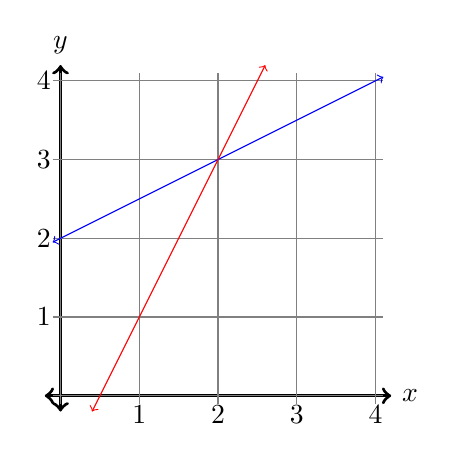
\begin{tikzpicture}
        \draw[very thick,<->] (-.2,0) -- (4.2,0) node[anchor=west] {$x$};
        \draw[very thick,<->] (0,-.2) -- (0,4.2) node[anchor=south] {$y$};
        \draw[gray,thin] (-.1,-.1) grid (4.1,4.1);
        \draw[blue,<->] plot[domain=-.1:4.1] (\x,.5*\x+2);
        \draw[red,<->] plot[domain=.4:2.6] (\x,2*\x-1);
        \foreach \x in {1,...,4} {
            \draw (\x,0) node[anchor=north] {$\x$};
            \draw (0,\x) node[anchor=east] {$\x$};
        }
    \end{tikzpicture}\end{center}
    The lines cross at the point $(2,3)$, so the solution is the $x$ value of this point: $x=2$.
    
    Next we solve symbolically/algebraically.
    \begin{align*}
        2x-1&=\frac{1}{2}x+2\\
        2x-\frac{1}{2}x-1&=2\\
        2x-\frac{1}{2}x&=2+1\\
        \frac{3}{2}x&=3\\
        x&=3\cdot\frac{2}{3}\\
        &=2.
    \end{align*}
    We got the same solution graphically and symbolically, $x=2$.
\end{solution}

\subsubsection{More complicated solutions}

So far, the equations we've see have all had solutions. In general, this doesn't always happen. There are three possiblilities for linear equations.
\begin{definition}{(Types of linear equation)}{def:types_of_linear_equation}
    There are three types of linear equation:
    \begin{itemize}
        \item Conditional equation: an equation with a single solution. Can be simplified to the form $x=a$ for some $a$.\\
        The equations we've seen so far have been conditional.
        \item Contradiction: an equation with no solutions.\\
        An equation is a contradiction if, when simplifying, you end up with a false statement such as $0=1$.
        \item Identity: an equation with infinitely many solutions.\\
        An equation is an identity if, when simplifying, you end up with a statement that is always true, like $0=0$ or $2x=2x$.
    \end{itemize}
\end{definition}

\begin{example}{(Textbook 2.2 ex 6)}{ex:2.2.6}
    Identify each equation as a contradiction, conditional equation, or identity.
    \begin{problem}
        \item $7+6x=2(3x+1)$
        \item $2x-5=3-(1+2x)$
        \item $2(5-x)-25=3(x-5)-5x$
    \end{problem}
\end{example}
\begin{solution}
    \begin{problem}
        \item We try to solve for $x$:
        \begin{align*}
            7+6x&=2(3x+1)\\
            7+6x&=6x+2\\
            7&=2.
        \end{align*}
        This is never true, so this equation is a contradiction.
        \item \begin{align*}
            2x-5&=3-(1+2x)\\
            2x-5&=3-1-2x\\
            4x-5&=2\\
            4x&=7\\
            x&=\frac{7}{4}.
        \end{align*}
        This is a single solution for $x$, so this equation is a conditional equation.
        \item \begin{align*}
            2(5-x)-25&=3(x-5)-5x\\
            10-2x-25&=3x-15-5x\\
            -2x-15&=-2x-15
        \end{align*}
        Since this is always true, this equation is an identity.
    \end{problem}
\end{solution}
% \includegraphics[width=6.5in]{Textbook_Mandatory_Examples/Exam1/2.2/2.2.6.png}

We can use the same operations we used for an equation of 1 variable to work with equations that have multiple variables. We isolate the variable of interest to express it in terms of the other variables.

\begin{example}{(Textbook 2.2 ex 12)}{ex:2.2.12}
    The area of a trapezoid with bases $a$ and $b$ and height $h$ is given by $a=\frac{1}{2}h(a+b)$. Solve this equation for $b$.
\end{example}
\begin{solution}
    We want to perform our allowed algebraic manipulations to get $b$ on one side.
    \begin{align*}
        A&=\frac{1}{2}h(a+b)\\
        2A&=h(a+b) && \text{multiply both sides by $2$}\\
        \frac{2A}{h}&=a+b && \text{divide both sides by $h$}\\
        \frac{2A}{h}-a&=b && \text{subtract $a$ from both sides}
    \end{align*}
    Now we have $b$ by itself on one side, so we have solved for $b$ in terms of the other variables.
\end{solution}
% \includegraphics[width=6.5in]{Textbook_Mandatory_Examples/Exam1/2.2/2.2.12.png}

\subsubsection{Word problems}

Now let's look at some examples using linear equations.

\begin{example}{(Textbook 2.2 ex 15)}{ex:2.2.15}
    A person 6 feet tall stands 17 feet from the base of a streetlight. If the person's shadow is 8 feet, estimate the height of the streetlight.
\end{example}
\begin{solution}
    \begin{minipage}{.36\textwidth}
        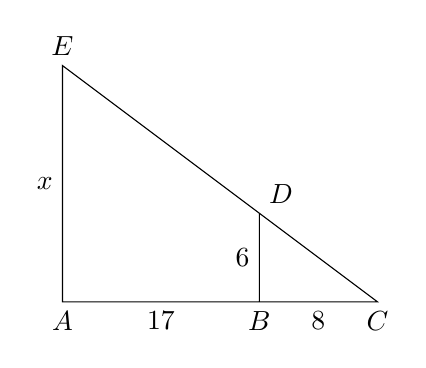
\begin{tikzpicture}
            \draw (2.5,0) node[anchor=north] {$B$} 
                -- node[below] {$8$} (4,0) node[anchor=north] {$C$}
                -- (2.5,4.5/4) node[anchor=south west] {$D$}
                -- (0,3) node[anchor=south] {$E$}
                -- node[left] {$x$} (0,0) node[anchor=north] {$A$}
                -- node[below] {$17$} (2.5,0) -- node[left] {$6$} (2.5,1.125);
        \end{tikzpicture}
    \end{minipage}
    \begin{minipage}{.63\textwidth}
        Let's begin by drawing a picture. We have two similar triangles:, as in the picture; the ratio of their base and horizontal sides will be the same, which we will use to find $x$.

        Since the ratio of the sides is the same, we know that \[\frac{6}{8}=\frac{x}{8+17}.\] Now we solve for $x$:
        \begin{align*}
            \frac{x}{25}&=\frac{3}{4}\\
            x&=25\cdot\frac{3}{4}\\
            &=\frac{75}{4}.
        \end{align*}
        We conclude that the lamppost is $\frac{75}{4}=18.75$ feet tall.
    \end{minipage}
\end{solution}
% \includegraphics[width=6.5in]{Textbook_Mandatory_Examples/Exam1/2.2/2.2.15.png}

\begin{example}{(Textbook 2.2 ex 13)}{ex:2.2.13}
    A large pump can empty a tank of gasoline in $5$ hours, and a smaller pump can empty the same tank in $9$ hours. If both pumps are used to empty the tank, how long will it take?
\end{example}
\begin{solution}
    Let $t$ be the number of hours it takes both pumps to fill up the tank. We want to come up with an equation which will let us solve for $t$.

    Since the large pump takes $5$ hours to empty the tank, each hour it empties $\frac{1}{5}$ of the tank. In $t$ hours, it will empty $t\cdot\frac{1}{5}$ of the tank.

    Similarly, since the small pump takes $9$ hours to empty the tank, each hour it empties $\frac{1}{9}$ of the tank and so in $t$ hours it empties $t\cdot\frac{1}{9}$ of the tank.

    Together, they empty the entire tank, which as a fraction is $\frac{1}{1}$. Therefore, we get the equation \[\frac{t}{5}+\frac{t}{9}=1.\]

    Now we solve for $t$:
    \begin{align*}
        \frac{t}{5}\cdot\frac{9}{9}+\frac{t}{9}\cdot\frac{5}{5}&=1\\
        \frac{9t}{45}+\frac{5t}{45}&=1\\
        \frac{14t}{45}&=1\\
        t&=\frac{45}{14}.
    \end{align*}
    Therefore, it takes $\frac{45}{14}\approx3.21$ hours for both pumps working together to empty the tank.
\end{solution}
% \includegraphics[width=6.5in]{Textbook_Mandatory_Examples/Exam1/2.2/2.2.13.png}

\begin{directions}
    Bonus example; do as time permits. Also, advise students that examples 14 and 16 in the book are worked examples of word problems that they can reference.
\end{directions}
\begin{example}{}{ex:density_linear_equation}
    Crushed sandstone has a density of 2.1 metric tons per meter cubed, while fill sand has a density of 1.4 metric tons per meter cubed. What percentage fill sand should you mix with crushed sandstone to get a fill material with a density of 1.5 tons per meter cubed?
\end{example}
\begin{solution}
    Let $x$ be the fraction of the mix that is fill sand. Then $1-x$ of the mix is crushed sandstone. Per 1 cubic meter of the mix, we have $x$ cubic meters of fill sand and $1-x$ cubic meters of crushed sandstone. Based on the densities of the materials, this will weigh \[x\cdot 1.4 + (1-x)\cdot2.1\text{ metric tons.}\]

    Since this is 1 cubic meter of material, we need it to weight $1.5$ metric tons. This gives us the equation \[1.4x+2.1(1-x)=1.5.\]

    Now we solve for $x$:
    \begin{align*}
        1.4x+2.1(1-x)&=1.5\\
        1.4x+2.1-2.1x&=1.5\\
        -.7x+2.1&=1.5\\
        -.7x&=-.6\\
        x&=\frac{.6}{.7}\\
        &=\frac{6}{7}.
    \end{align*}
    Now we know what fraction of the mix is fill sand; we want to convert this to a percentage. As a decimal, $\frac{6}{7}=.\overline{857142}$, so as a percent this is approximately $85.71\%$ of the mixture.
\end{solution}

\end{document}